\section{Sensor}
Sensoren som bliver beskrevet i hardware afsnittet skal kommunikere med arduino boardet. Dette kræver nogle trin som kan findes i databladet til sensoren. På figur \ref{sensor_kom} ses et overblik over funktioner gruppen har lavet, som skal til for at aflæse sensoren. Disse funktioner er konstrueret ved at anvende databladet hvor det ses at tre trin skal følges til punkt og prikke for at kunne tilgå sensoren. De tre trin er en initialization, ROM command of function command.
\\
\\
I databladet ses et stort flowchart over de forskellige måde sensoren kan tilgåes, ud fra denne har vi konstrueret en mindre version for det minimum vi skal bruge for at kunne tilgå sensoren. Denne kan ses på figur 

\begin{figure}[h!]
  \centering
  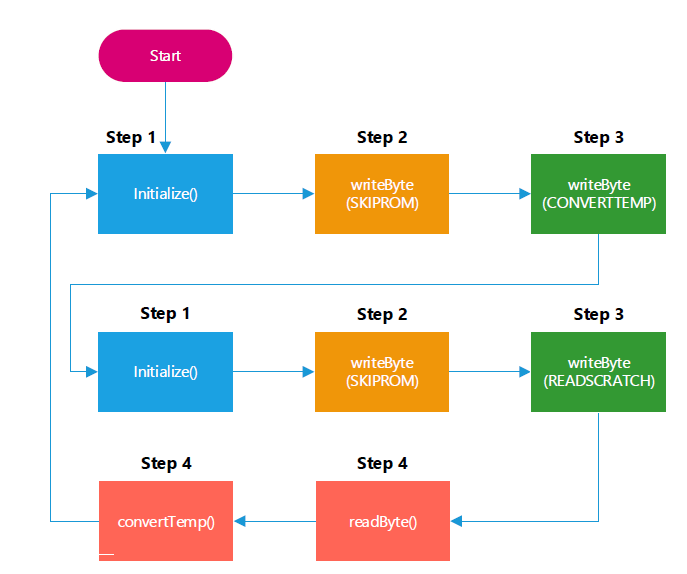
\includegraphics[width=0.8\textwidth]{figures/sensor_communication.png}
  \caption{Kommunikation med sensor.}
  \label{sensor_kom}
\end{figure}
\fxnote{ret størrelse til på alle billeder(noget der skal gøres til sidst!)}

\newpage
\subsection{Initialize}
Initialisering af sensoren gøres ved at sætte 1-wire forbindelsen til sensorsen til low i et specifikt stykke tid.

\begin{figure}[h!]
  \centering
  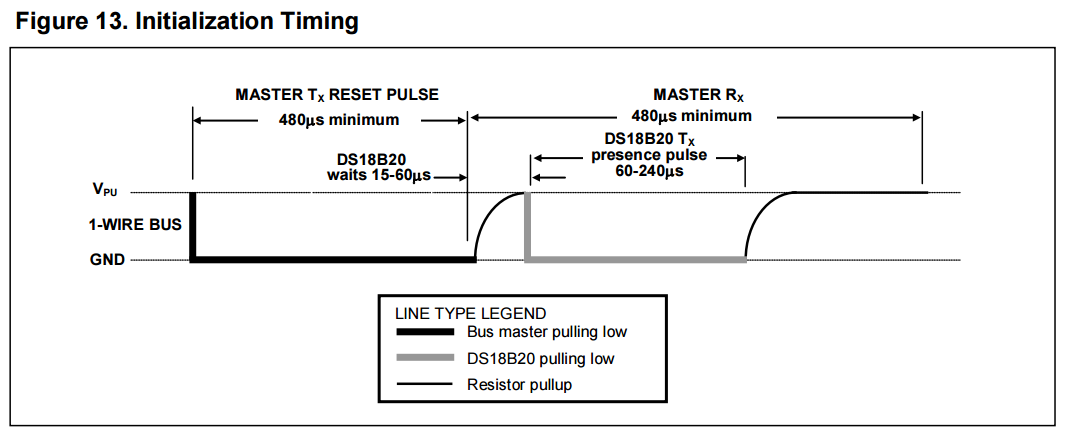
\includegraphics[width=0.5\textwidth]{figures/Initialization_timing.png}
  \caption{Fra datablad om hvordan sensor skal initialiseres.}
  \label{sensor_kom}
\end{figure}

Fra databladet ses det at 1-wire forbindelsen skal have en reset pulse i minimum 480$\mu$S og en presence pulse i 60 til 240$\mu$S. Dette gøres ved at sende et low signal som reset pulse og derefter sætte forbindelsen i tri-state og pull-up modstanden trækker signalet højt. 

I koden gøres dette ved at bruge digitalWrite til low i kombination med et delay på 500$\mu$S. Derefter sættes pinMode til input og et delay på 500$\mu$S anvendes igen. Dette kan ses på figur \ref{sensor_kode}.

\begin{figure}[h!]
  \centering
  \includegraphics[width=1\textwidth]{figures/Init.png}
  \caption{Initialisering kode.}
  \label{sensor_kode}
\end{figure}